This sections evaluates the performance of proposed methodology in estimating correspondences of human poses in-the-wild. Results for quantitative an qualitative experiments are reported. Experiments \ref{exp:internal} investigate the accuracy of estimating dense correspondences of non-rigid deformable objects, and the impact of annotating outlines of human poses instead of annotating skeletons. Experiments \ref{exp:benchmark} compare the joints localisation accuracy of our skeleton prediction from outline fitting with respect to that of state-of-the-art human pose estimation algorithms in-the-wild. Note that all results reported in this section were obtained by fitting Patch AAM using the fast version of the Simultaneous Inverse Compositional algorithm (Fast-SIC) originally proposed by the authors of \cite{Papandreou2008}. For further experimental results and visualisations please refer to our supplementary material.

\subsection{Databases \& Error Metrics}
There are significant numbers of datasets exist for human pose estimation, where FLIC\cite{}, BBC Pose\cite{}, Fashion Pose\cite{} and MPII\cite{} attracted most public attention. In our work, we reported our performance comparison on BBC Pose Dataset\cite{}, which has relatively most consistent skeleton annotation among the others. 

The training of dense Active Appearance Models (dAAMs) for upper body involves manual outline annotation from a combination of datasets, including H3D\cite{}, Microsoft COCO\cite{}, MPII\cite{}, Fashion Pose\cite{}, FLIC\cite{} and BBC Poses\cite{}. The training set contains 891 training images from where 500 are annotated with outline manually. A dAAMs is built from 500 training images thereby produces dense correspondences for generating sparse outline annotation. A Patch AAM is build from sparse annotations before fitting to 391 images. Manual minor correction are required for putting those fitted image to training set. The final Patch AAM is built from 891 images and validated on validation set given by BBC Pose.



\subsection{Internal Evaluation}
\label{exp:internal}

\begin{figure}[t!]
    \centering
    \begin{subfigure}[b]{0.23\textwidth}
            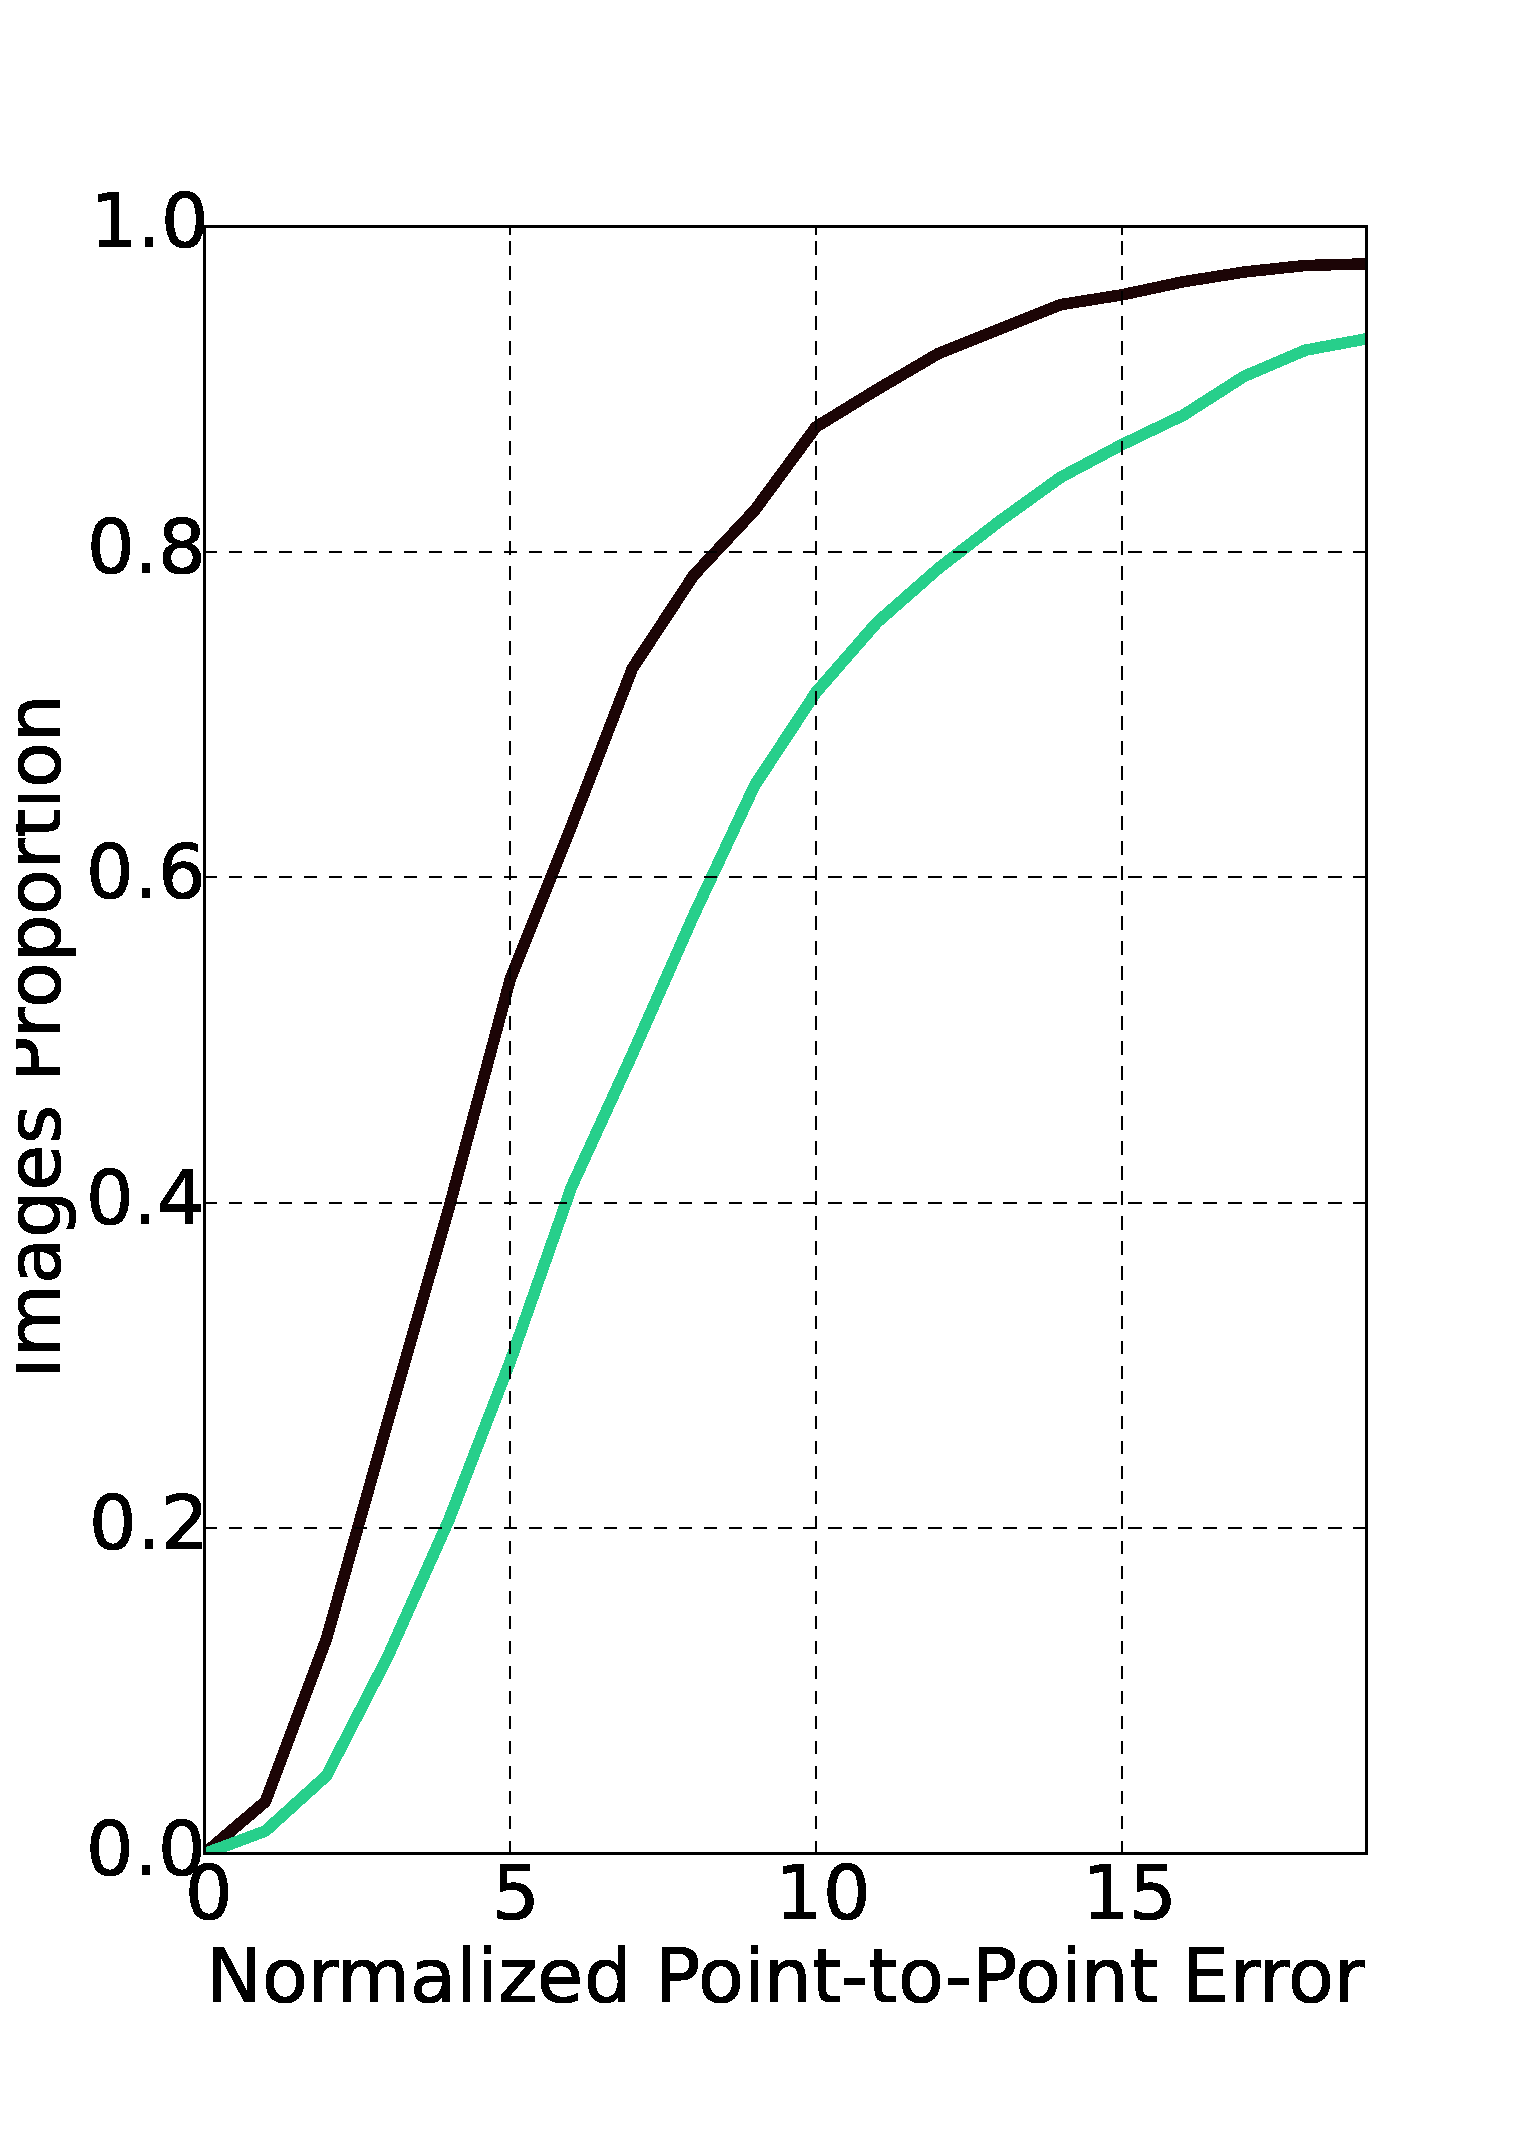
\includegraphics[width=\textwidth]{resources/HandBenchmark/elbow_joints}
    \end{subfigure}
    \hfill
    \begin{subfigure}[b]{0.23\textwidth}
            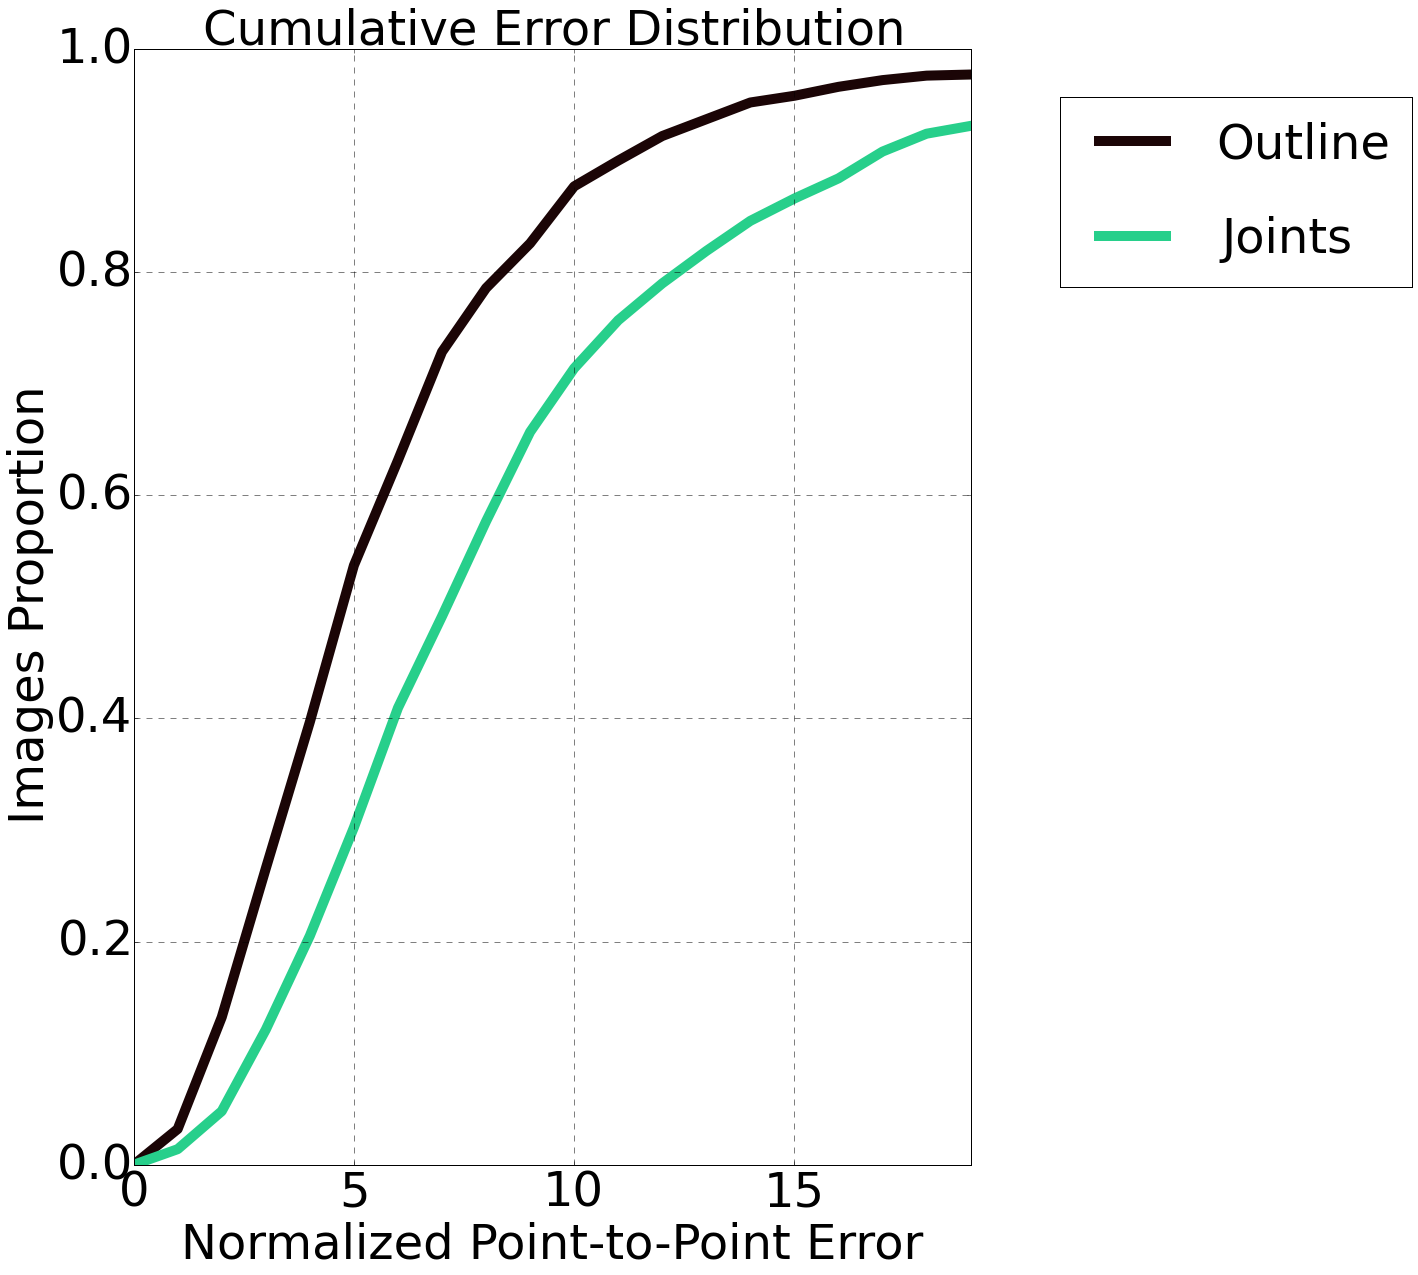
\includegraphics[width=\textwidth]{resources/HandBenchmark/wrist_joints}
    \end{subfigure}
    \caption{Hand Benchmark.}
    \label{fig:internal_benchmark}
\end{figure}

\subsection{Benchmark Against State-of-the-art}
\label{exp:benchmark}

\begin{figure}[t!]
    \centering
    \begin{subfigure}[b]{0.23\textwidth}
            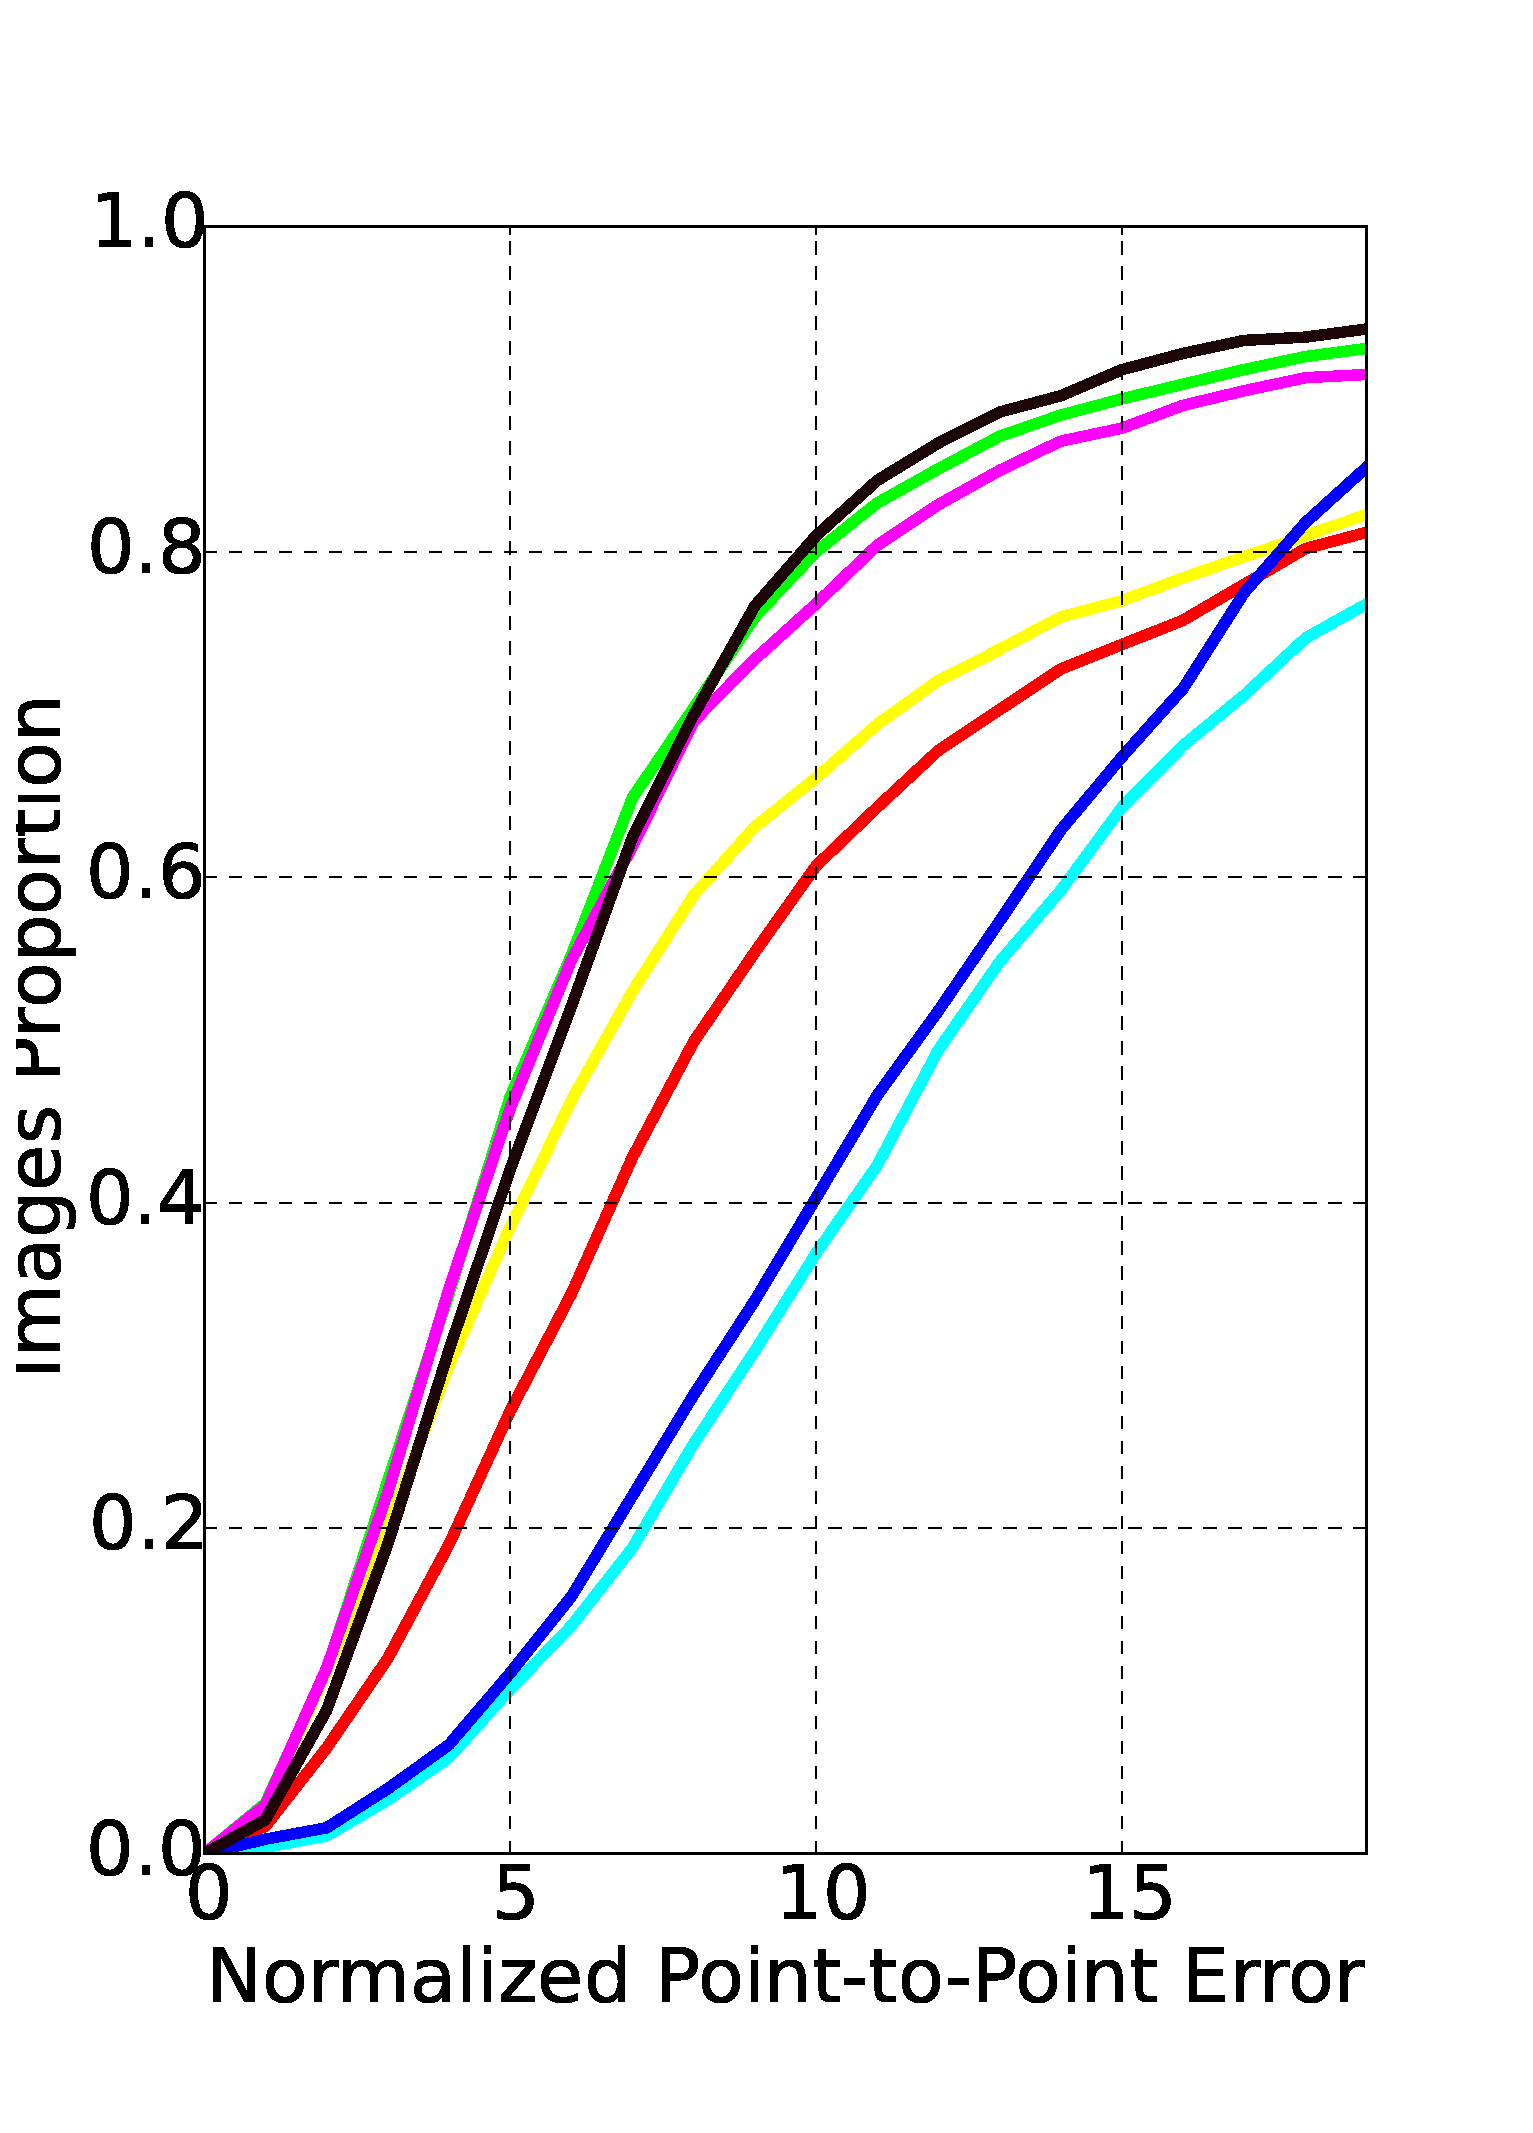
\includegraphics[width=\textwidth]{resources/HandBenchmark/elbow}
    \end{subfigure}
    \hfill
    \begin{subfigure}[b]{0.23\textwidth}
            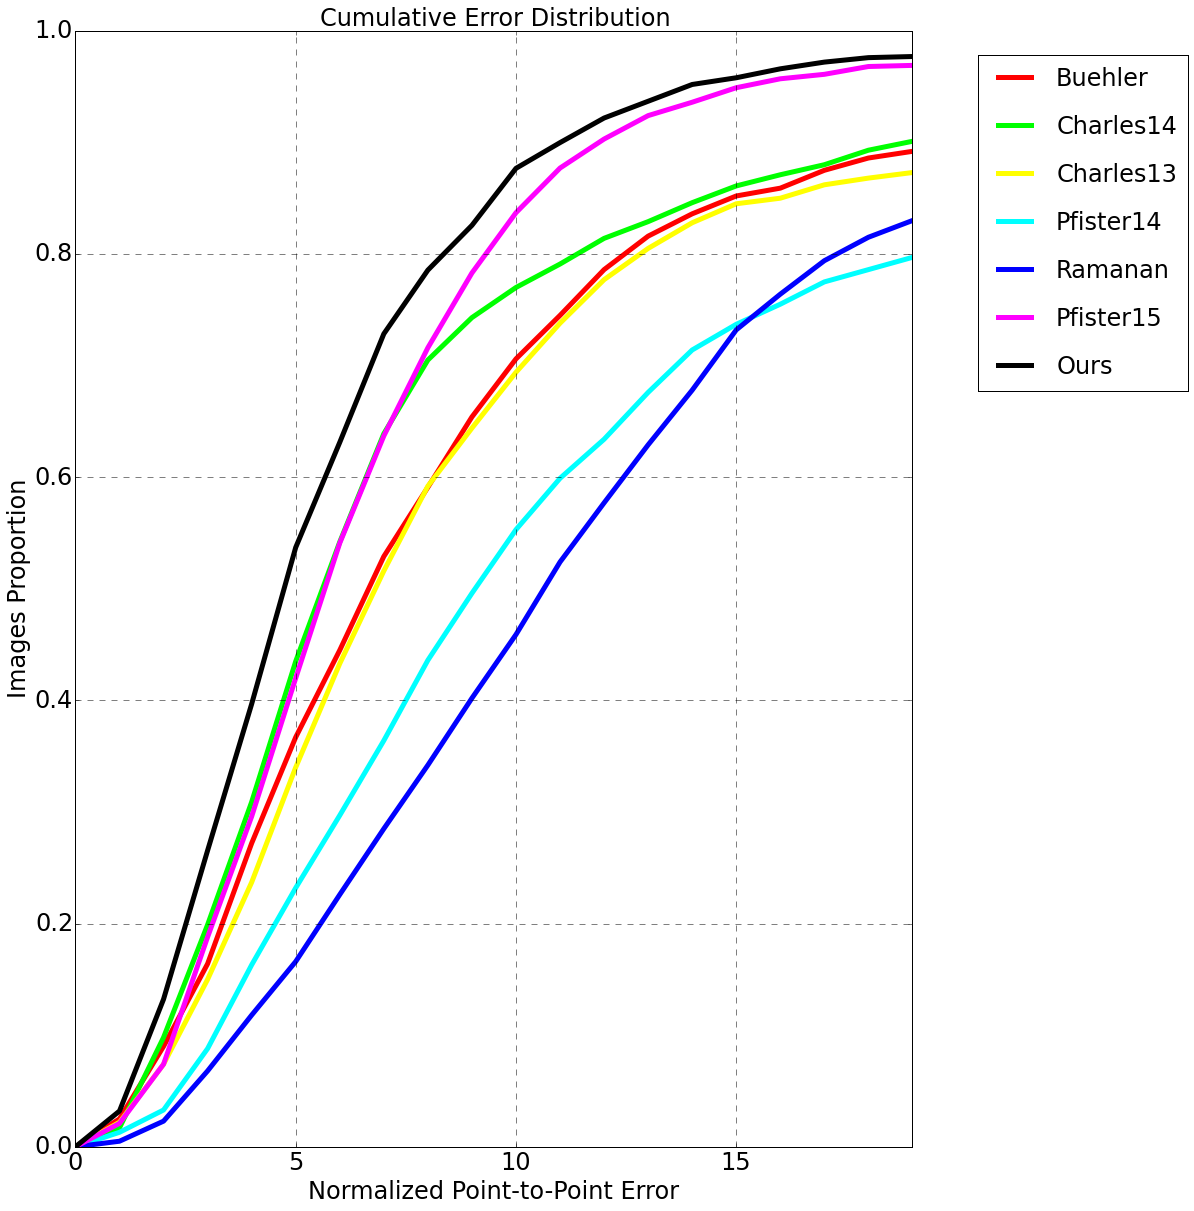
\includegraphics[width=\textwidth]{resources/HandBenchmark/wrist}
    \end{subfigure}
    \caption{Hand Benchmark.}
    \label{fig:hand_benchmark}
\end{figure}


\subsection{Qualitative Results}
\label{exp:qualitative}
